%20 min preso!
\documentclass[xcolor=table]{beamer}
\usepackage{beamerthemesplit}
\usepackage{wrapfig}
\usetheme{SPbGU}
\usepackage{pdfpages}
\usepackage{amsmath}
\usepackage{cmap}
\usepackage[T2A]{fontenc}
\usepackage[utf8]{inputenc}
\usepackage[english]{babel}
\usepackage{indentfirst}
\usepackage{amsmath}
\usepackage{tikz}
\usepackage{multirow}
\usepackage[noend]{algpseudocode}
\usepackage{algorithm}
\usepackage{algorithmicx}
\usepackage{fancyvrb}
\usetikzlibrary{calc}
\usetikzlibrary{shapes,arrows}
\usetikzlibrary{arrows,automata}
\usetikzlibrary{positioning}
\usetikzlibrary{fit}

\usepackage{tabularx}
\newcolumntype{Y}{>{\raggedleft\arraybackslash}X}

\renewcommand{\thealgorithm}{}

\newtheorem{mytheorem}{Theorem}
\renewcommand{\thealgorithm}{}

\newcommand{\tikzmark}[1]{\tikz[overlay,remember picture] \node (#1) {};}
\def\Put(#1,#2)#3{\leavevmode\makebox(0,0){\put(#1,#2){#3}}}

\newcommand{\ltz}{$< 1$}


\tikzset{
    state/.style={
           rectangle,
           rounded corners,
           draw=black, very thick,
           minimum height=2em,
           inner sep=2pt,
           text centered,
           },
}

\beamertemplatenavigationsymbolsempty

\title[Kronecker Product CFPQ]{Context-Free Path Querying by Kronecker Product}
%\subtitle[YaccConstructor]{Parsing techniques for graph analysis}
% То, что в квадратных скобках, отображается в левом нижнем углу.
\institute[JetBrains Research]{
JetBrains Research, Programming Languages and Tools Lab  \\
Saint Petersburg University
}

% То, что в квадратных скобках, отображается в левом нижнем углу.
\author[Rustam Azimov]{Egor Orachev, Ilya Epelbaum, \\ Semyon Grigorev, \textbf{Rustam Azimov}}

\date{August 26, 2020}

\begin{document}
{
\begin{frame}[fragile]
  \begin{table}
  \centering
  \begin{tabularx}{\linewidth}{YcX}
    
\includegraphics[height=1.5cm]{pictures/jetbrainsResearch.pdf} \hfill
    & \begin{minipage}[t]{0.3\textwidth}\center \vspace{-1cm}  ADBIS 2020
      \end{minipage}
    & \hfill 
\includegraphics[height=1.5cm]{pictures/SPbGU_Logo.png}
  \end{tabularx}
  \end{table}
  \titlepage
\end{frame}
}

\begin{frame} \frametitle{Context-Free Path Querying}
  \begin{minipage}[m]{0.45\linewidth}
  \raisebox{-0.5\totalheight}{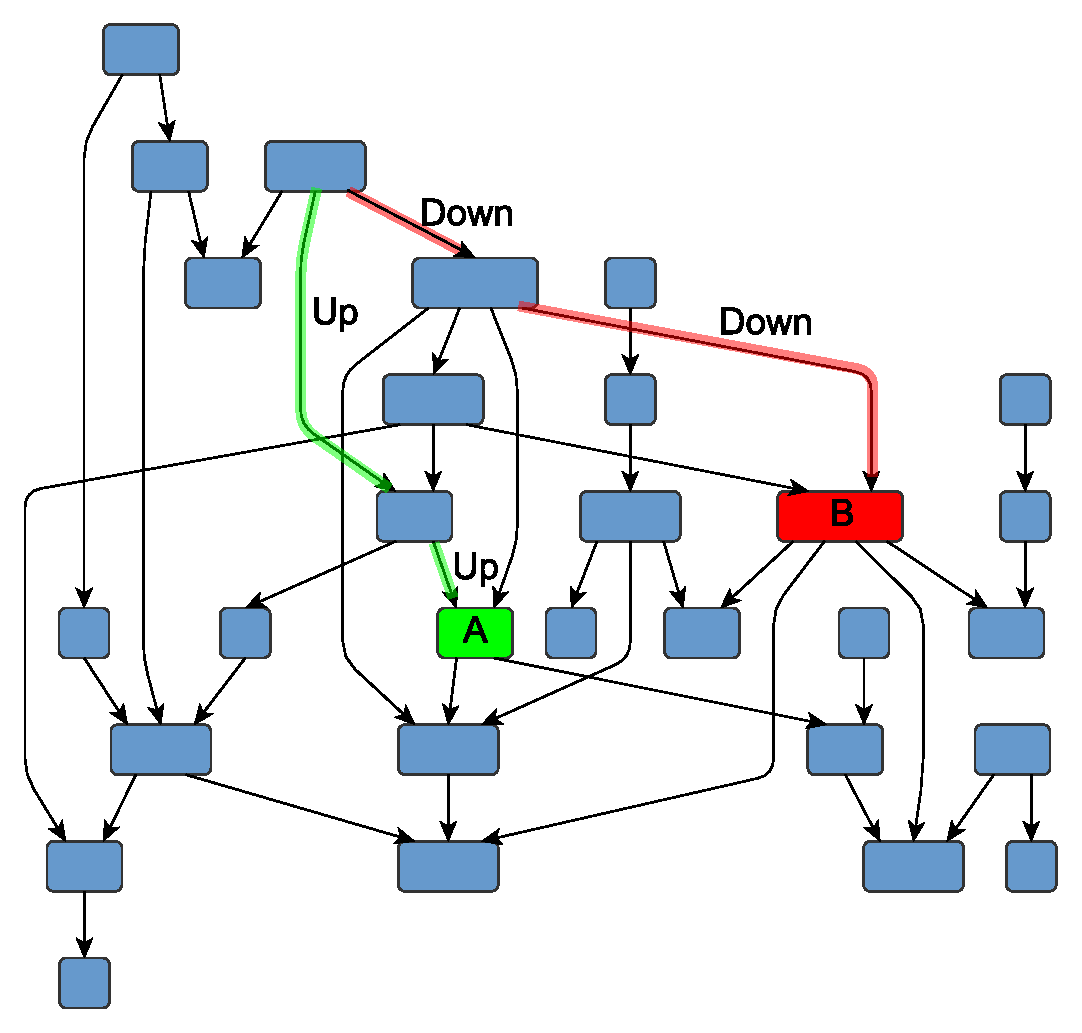
\includegraphics[width=\textwidth]{pictures/hierarchical.pdf}}
  \end{minipage}\hfill
  \begin{minipage}[m]{0.5\linewidth}
  Navigation through a graph
  \begin{itemize}
        \item Are nodes A and B on the same level of hierarchy?
        \item Is there a path of form $\textbf{Up}^n \, \textbf{Down}^n$?
        \item Find all paths of form $\textbf{Up}^n \, \textbf{Down}^n$ which start from the~node A
  \end{itemize}

  \end{minipage}

  \end{frame}

%  \begin{frame}[fragile] \frametitle{Applicatipons}
%    \begin{itemize}
%      \item Static code analysis
%      \item Graph database querying
%      \item RDF analysis
%    \end{itemize}
%  \end{frame}

  \begin{frame}[fragile]
    \frametitle{CFPQ: Query Semantics}
    \begin{itemize}
      \item $\mathbb{G} = (\Sigma, N, P)$ --- context-free grammar in normal form
      \begin{itemize}
        \item $A \rightarrow B C$, where $A, B, C \in N$
        \item $A \rightarrow x$, where $A \in N, x \in \Sigma \cup \{\varepsilon\}$
        \item $L(\mathbb{G},A) = \{ \omega \mid A \Rightarrow^* \omega \}$
      \end{itemize}
      \pause
      \item $G = (V,E,L)$ --- directed graph
        \begin{itemize}
          \item $v \xrightarrow{l} u \in E$
          \item $L \subseteq \Sigma$
        \end{itemize}
        \pause
      %\item $p = v_0 \xrightarrow{l_0} v_1 \xrightarrow{l_1} \cdots \xrightarrow{l_{n-2}} v_{n-1} \xrightarrow{l_{n-1}} v_n$ --- path in $G$
      \item $\omega(\pi) = \omega(v_0 \xrightarrow{l_0} v_1 \xrightarrow{l_1} \cdots \xrightarrow{l_{n-2}} v_{n-1} \xrightarrow{l_{n-1}} v_n) = l_0 l_1 \cdots l_{n-1}$
      \pause
      \item $R_A = \{ (n, m) \mid \exists n \pi m$, such that $\omega(\pi) \in L(\mathbb{G},A)\}$
    \end{itemize}
  \end{frame}

  \begin{frame}[fragile] \frametitle{CFPQ: Original Matrix-Based Algorithm}
    	\begin{algorithm}[H]
    		\begin{algorithmic}[1]
    			\caption{Context-free path querying algorithm}
    			\label{lst:algo1}
    			\Function{evalCFPQ}{$D=(V,E,L), G=(\Sigma,N,P)$}
    			\State{$n \gets$ |V|}
    			\State{$T \gets \{T^{A_i} \mid A_i \in N, T^{A_i}$ is a matrix $n \times n$, $T^{A_i}_{k,l} \gets$ \texttt{false}\} }
    			\ForAll{$(i,x,j) \in E$, $A_k \mid A_k \to x \in P$}
    			%\Comment{Matrices initialization}
    			%\For{$A_k \mid A_k \to x \in P$}
    			{$T^{A_k}_{i,j} \gets \texttt{true}$}
    			%\EndFor
    			\EndFor
    			\ForAll{$A_k \mid A_k \to \varepsilon \in P$}
    			\ForAll{$i \in \{0,\ldots ,n-1\}$}
    			{$T^{A_k}_{i,i} \gets \texttt{true}$}
    			\EndFor
    			\EndFor
    			
    			\While{any matrix in $T$ is changing}
    			%\Comment{Transitive c	losure calculation}
    			\For{$A_i \to A_j A_k \in P$}
    			{ $T^{A_i} \gets T^{A_i} + (T^{A_j} \times T^{A_k})$ } 
    			\EndFor
    			\EndWhile
    			\State \Return $T$
    			\EndFunction
    		\end{algorithmic}
    	\end{algorithm}
  \end{frame}

\begin{frame}[fragile]
\frametitle{CFPQ: Grammar Transformation}
\begin{itemize}
	\item $\mathbb{G} = (\Sigma, N, P)$ --- context-free grammar in general form
	\begin{itemize}
		\item $A \rightarrow \alpha$, where $A \in N, \alpha \in (N \cup \Sigma \cup \{\varepsilon\})^*$
	\end{itemize}
	\pause
	\item Every context-free grammar can be transformed to binary normal form
	\pause
	\item The transformation takes time and can lead to a significant grammar size increase
	
\end{itemize}
\end{frame}

\begin{frame}[fragile] \frametitle{Research Questions}
\begin{itemize}
	\item Can we create the matrix-based CFPQ algorithm that does not require grammar transformation?
	\item What matrix operations should be used?
	\item Does using matrix optimizations still significantly increases performance?
\end{itemize}
\end{frame}

\begin{frame}[fragile] \frametitle{Recursive State Machines (RSM)}
\begin{itemize}
	\item RSM behaves as a set of finite state machines (FSM)
	\item Each FSM (box) works almost the same as a classical FSM, but it also handles additional recursive calls and employs an implicit call stack to call one component from another and then return execution flow back
	\item Any CFG can be easily encoded by an RSM with one box per nonterminal
\end{itemize}

\begin{figure}[h]
	\begin{tikzpicture}[shorten >=1pt,auto]
	\node[state, initial] (q_0)   {$q_S^0$};
	\node[state] (q_1) [right=of q_0] {$q_S^1$};
	\node[state] (q_2) [right=of q_1] {$q_S^2$};
	\node[state, accepting] (q_3) [right=of q_2] {$q_S^3$};
	\path[->]
	(q_0) edge node {a} (q_1)
	(q_1) edge node {S} (q_2)
	(q_2) edge node {b} (q_3)
	(q_1) edge [bend left, above]  node {b} (q_3);
	\node[draw=black, fit= (q_0) (q_1) (q_2) (q_3), xshift=-4.5ex,inner sep=0.75cm, label=Box S] {};
	\end{tikzpicture}
	\centering
	\caption{The RSM for grammar with rules $S \to a S b \mid a b$}
\end{figure}

\end{frame}

\begin{frame}[fragile] \frametitle{Kronecker Product}
\begin{itemize}
	\item Kronecker product $A \otimes B$ for matrix $A$ of size $m \times n$ and matrix $B$ of size $p \times q$
	\begin{itemize}
		\item Multiply each element of $A$ and the matrix $B$
		\item As a result we have $pm \times qn$ block matrix
	\end{itemize}
	\item We need to intersect the FSMs from RSM generated by the context-free grammar and FSM generated by the graph
	\item Kronecker product can be used for constructing such intersections
\end{itemize}

\end{frame}

\begin{frame}[fragile] \frametitle{Kronecker Product Based CFPQ Algorithm}

\begin{algorithm}[H]
	{\footnotesize
\begin{algorithmic}[1]
	\caption{Kronecker product based CFPQ}
	\label{tensor:cfpq}
	\Function{contextFreePathQuerying}{G, $\mathcal{G}$}
	% Input data preparation
	\State{$R \gets$ Recursive automata for $G$}
	\State{$M_1, M_2 \gets$ Adjacency matrices for $R$ and $\mathcal{G}$}
	% Eps-transition handling for graph
	\For{$s \in 0..dim(M_1)-1$}
	\For{$i \in 0..dim(M_2)-1$}
	\State{$M_2[i,i] \gets M_2[i,i] \cup \textit{getNonterminals}(R,s,s)$}
	\EndFor
	\EndFor
	\While{Matrix $M_2$ is changing}
	\State{$M_3 \gets M_1 \otimes M_2$}
	\Comment{Evaluate Kronecker product}
	\State{$C_3 \gets \textit{transitiveClosure}(M_3)$}
	\State{$n \gets$ dim($M_3)$}
	\Comment{Matrix $M_3$ size = $n \times n$}
	% Add non-terminals (possibly new)
	\For{$i \in 0..n-1$}
	\For{$j \in 0..n-1$}
	\If{$C_3[i,j]$}
	\State{$s, f \gets \textit{getStates}(C_3,i,j)$}
	\If{$\textit{getNonterminals}(R,s,f) \neq \emptyset$}
	\State{$x, y \gets \textit{getCoordinates}(C_3,i,j)$}
	\State{$M_2[x,y] \gets M_2[x,y] \cup \textit{getNonterminals}(R,s,f)$}
	\EndIf
	\EndIf
	\EndFor
	\EndFor
	\EndWhile
	\State \Return $M_2$
	\EndFunction
\end{algorithmic}
}
\end{algorithm}


\end{frame}

  \begin{frame}[fragile] \frametitle{Kronecker Product Based CFPQ Algorithm: Technical Details}
    \begin{itemize}
      \item We can use the sparse and block nature of the obtained matrices to apply wide class of optimizations
      \item We can operate over Boolean matrices
      \item We still can use existing high-performance math libraries for intersection if they provide a satisfying operation of element-wise multiplication
    \end{itemize}
  \end{frame}

\begin{frame}[fragile] \frametitle{Implementations}

\begin{itemize}
	\item $\textbf{Kron}$ --- implementation of the proposed algorithm using \textbf{SuiteSparse} C implementation of \textbf{GraphBLAS} API, which provides a set of sparse matrix operations
	\pause
	\item We compare our implementation with $\textbf{Orig}$ --- the best CPU implementations of the original matrix-based algorithm using M4RI library with sparse matrix representation
\end{itemize}
\end{frame}

\begin{frame} \frametitle{Evaluation}
\begin{itemize}
	\item OS: Ubuntu 18.04
	\item CPU: Intel(R) Core(TM) i7-4790 CPU 3.60GHz
	\item RAM: DDR4 32 Gb
\end{itemize}
\end{frame}


\begin{frame}[fragile] \frametitle{Evaluation results\footnote{Queries are based on the context-free grammars for 
		nested parentheses} \footnote{Time is measured in seconds}}
\begin{center}
	\tikzmark{yyy}{
	}
 {\small
 \setlength{\tabcolsep}{0.35em}
 			\centering
 			\label{tbl:tableRDF}
 			%\rowcolors{1}{}{lightgray}
 			\begin{tabular}{| c | p{1.6cm} | c | c | c | c || c | p{0.8cm} | c | c | c | c |}
 				\hline
 				&  Graph              & \#V & \#E  & $Kron$  & $Orig$ &  & Graph & \#V & \#E     & $Kron$    & $Orig$ \\
 				\hline
 				\hline
 				\parbox[t]{2mm}{\multirow{11}{*}{\rotatebox[origin=c]{90}{RDF}}}
 				& \small{generations}                 & 129 & 351     & 0.04  & 0.03 &
 				\parbox[t]{2mm}{\multirow{2}{*}{\rotatebox[origin=c]{90}{RDF}}} & \small{core}                        & 1323 & 8684   & 0.28  &  0.12   \\
 				& \small{travel}                      & 131 & 397     & 0.05  & 0.05 & & \small{pways}                    & 6238 & 37196  & 4.88 &   0.18      \\\cline{7-12}
 				& \small{skos}                        & 144 & 323     & 0.02  & 0.04 &
 				\parbox[t]{2mm}{\multirow{5}{*}{\rotatebox[origin=c]{90}{Worst case}}} & $WC_1$& 64 & 65 & 0.03 & 0.04      \\
 				& \small{unv-bnch}                    & 179 & 413     & 0.05  & 0.04 & & $WC_2$ & 128 & 129 & 0.16 & 0.23      \\
 				& \small{foaf}                        & 256 & 815     & 0.07  & 0.02  & & $WC_3$ & 256 & 257 & 0.96 & 1.99    \\
 				& \small{atm-prim}                    & 291 & 685     & 0.24   & 0.02 & & $WC_4$ & 512 & 513 & 7.14 & 23.21      \\
 				& \small{ppl\_pets}                & 337 & 834     & 0.18  & 0.03 & & $WC_5$ & 1024& 1025&  121.99 & 528.52      \\ \cline{7-12}
 				& \small{biomed}                      & 341 & 711     & 0.24  & 0.05 &
 				\parbox[t]{2mm}{\multirow{4}{*}{\rotatebox[origin=c]{90}{Full}}} & $F_1$ & 100 & 100 & 0.17 &  0.02     \\
 				& \small{pizza}                       & 671 & 2604    & 1.14  & 0.08 & & $F_2$ & 200 & 200 & 1.04 & 0.03        \\
 				& \small{wine}                        & 733 & 2450    & 1.71  & 0.06 & & $F_3$ & 500 & 500 & 18.86  & 0.03   \\
 				& \small{funding}                     & 778 & 1480    & 0.43  & 0.07  & & $F_4$ & 1000 & 1000& 554.22 & 0.07       \\
 				\hline
 			\end{tabular}
 	}
\end{center} 
%\pause
%\onslide<2>{\tikz[overlay,remember picture]{\draw[draw=red,thick,fill opacity=0.2] ($ (yyy) + (2,-0.85)$) rectangle ($ (yyy) + (7.18,-1.6)$);}}
%\pause
%\onslide<3>{\tikz[overlay,remember picture]{\draw[draw=red,thick,fill opacity=0.2] ($ (yyy) + (4.6,1.2)$) rectangle ($ (yyy) + (5.3,-1.58)$);}}
%\pause
%\onslide<4>{\tikz[overlay,remember picture]{\draw[draw=red,thick,fill opacity=0.2] ($ (yyy) + (5.4,1.2)$) rectangle ($ (yyy) + (6.1,-1.58)$);}}
%\pause
%\onslide<5>{\tikz[overlay,remember picture]{\draw[draw=red,thick,fill opacity=0.2] ($ (yyy) + (9.2,1.2)$) rectangle ($ (yyy) + (9.9,-1.58)$);}}
\end{frame}

\begin{frame}[fragile] \frametitle{Conclusion}
  \begin{itemize}
  	\item We show that in some cases our algorithm outperforms the original matrix-based algorithm
  	\pause
    \item We still can use existing high-performance libraries for matrix operations
    \pause
    \item The idea of the proposed algorithm looks viable
  \end{itemize}
  \pause
  \begin{itemize}
    \item Dataset is published: both graphs and queries
    \begin{itemize}
    	\item Link: \url{https://github.com/JetBrains-Research/CFPQ_Data}
    \end{itemize}
    
    %\item Implementations are available on GitHub
    %\begin{itemize}
    %	\item Link: \url{https://github.com/YaccConstructor/RedisGraph}
    %\end{itemize}
    
  \end{itemize}
\end{frame}

\begin{frame}[fragile] \frametitle{Future Research}
  \begin{itemize}
  	\item Improve our implementation to make it applicable for real-world graphs analysis
  	\pause
  	\item Investigate such formal properties of the proposed algorithm as time and space complexity
  	\pause
  	\item Analyze how the behavior depends on the query type and its form
  	\begin{itemize}
  		\item Analyze regular path queries evaluation and context-free path queries in the form
  		of extended context-free grammars (ECFG)
  	\end{itemize}
  	\pause	
    \item Compare our algorithm with the matrix-based one
    in cases when the size difference between Chomsky Normal Form and ECFG
    representation of the query is significant.
    \pause
    \item Extend our algorithm to single-path and all-path
    query semantics
\end{itemize}
\end{frame}

\begin{frame}
\frametitle{Contact Information}
\begin{itemize}
  \item Semyon Grigorev:
    \begin{itemize}
      \item \href{mailto:s.v.grigoriev@spbu.ru}{s.v.grigoriev@spbu.ru}
      \item \href{mailto:Semen.Grigorev@jetbrains.com}{Semen.Grigorev@jetbrains.com}
    \end{itemize}
  \item Rustam Azimov:
  \begin{itemize}
  	\item \href{mailto:rustam.azimov19021995@gmail.com}{rustam.azimov19021995@gmail.com}
  	\item \href{mailto:Rustam.Azimov@jetbrains.com}{Rustam.Azimov@jetbrains.com}
  \end{itemize}
  \item Egor Orachev: \href{mailto:egor.orachev@gmail.com}{egor.orachev@gmail.com}
  \item Ilya Epelbaum: \href{mailto:iliyepelbaun@gmail.com}{iliyepelbaun@gmail.com}
\vspace{0.5cm}
  \item Dataset: \href{https://github.com/JetBrains-Research/CFPQ_Data}{https://github.com/JetBrains-Research/CFPQ\_Data}
   %\item Algorithm implementations: \href{https://github.com/YaccConstructor/RedisGraph}{https://github.com/YaccConstructor/RedisGraph}
\end{itemize}
\vspace{0.1cm}
\center{\huge{Thanks!}}
\end{frame}
\end{document}
